\documentclass{jib}
\newlength{\platz}
\setlength{\platz}{15pt}
\RequirePackage{listings}
\lstset{%
  basicstyle=\ttfamily,
  fontadjust,
  flexiblecolumns=true,
  frame=L,
  xleftmargin=15pt,
  framesep=5pt,
  emphstyle=\rmfamily\itshape}

\usepackage{pdfpages}

%%%%%%%%%%%%%%%%%%%%%%%%%%%%%%%%%%%%%%%%%%%%%%%%%%%%%%%%%%
% JIB Header/Footer
%%%%%%%%%%%%%%%%%%%%%%%%%%%%%%%%%%%%%%%%%%%%%%%%%%%%%%%%%%
\jibvolume{XX} % insert volume
\jibissue{X}   % insert issue
\jibpages{XXX} % insert article ID
\jibyear{XXXX} % insert year
\makeHeaderFooter{} % leave as is
%%%%%%%%%%%%%%%%%%%%%%%%%%%%%%%%%%%%%%%%%%%%%%%%%%%%%%%%%%

\begin{document}

%%%%%%%%%%%%%%%%%%%%%%%%%%%%%%%%%%%%%%%%%%%%%%%%%%%%%%%%%%
%
% Title Page
%
%%%%%%%%%%%%%%%%%%%%%%%%%%%%%%%%%%%%%%%%%%%%%%%%%%%%%%%%%%

\begin{jibtitlepage}

\jibtitle{SBML Level 3 package: Multistate, Multicomponent and Multicompartment Species, Version 1 Release 3}

\jibauthor{%
  Fengkai Zhang\iref{niaid},
  Martin Meier-Schellersheim\iref{niaid}%
}

\addjibinstitution{niaid}{
National Institute of Allergy and Infectious Disease (NIAID), \\
National Institutes of Health (NIH), \\
Bethesda, Maryland, USA
}

\end{jibtitlepage}

% The abstract

\begin{abstract}
Rule-based modeling is an approach that permits constructing reaction
networks based on the specification of rules for molecular
interactions and transformations. These rules can encompass details
such as the interacting sub-molecular domains (components) and the
states such as phosphorylation and binding status of the involved
components. Fine-grained spatial information such as the locations of
the molecular components relative to a membrane (e.g. whether a
modeled molecular domain is embedded into the inner leaflet of the
cellular plasma membrane) can also be provided. Through wildcards
representing component states entire families of molecule complexes
sharing certain properties can be specified as patterns. This can
significantly simplify the definition of models involving species with
multiple components, multiple states and multiple compartments. 
The SBML Multi Package (Multistate, Multicomponent and
Multicompartment Species Package for SBML Level 3) extends the SBML
core with the ``type'' concept in the Species and Compartment classes
and therefore reaction rules may contain species that can be patterns
and be in multiple locations in reaction rules. 
Multiple software tools such as Simmune and BioNetGen support the SBML
Multi package that thus also becomes a medium for exchanging rule-based models.

\end{abstract}

% Include your PDF document
%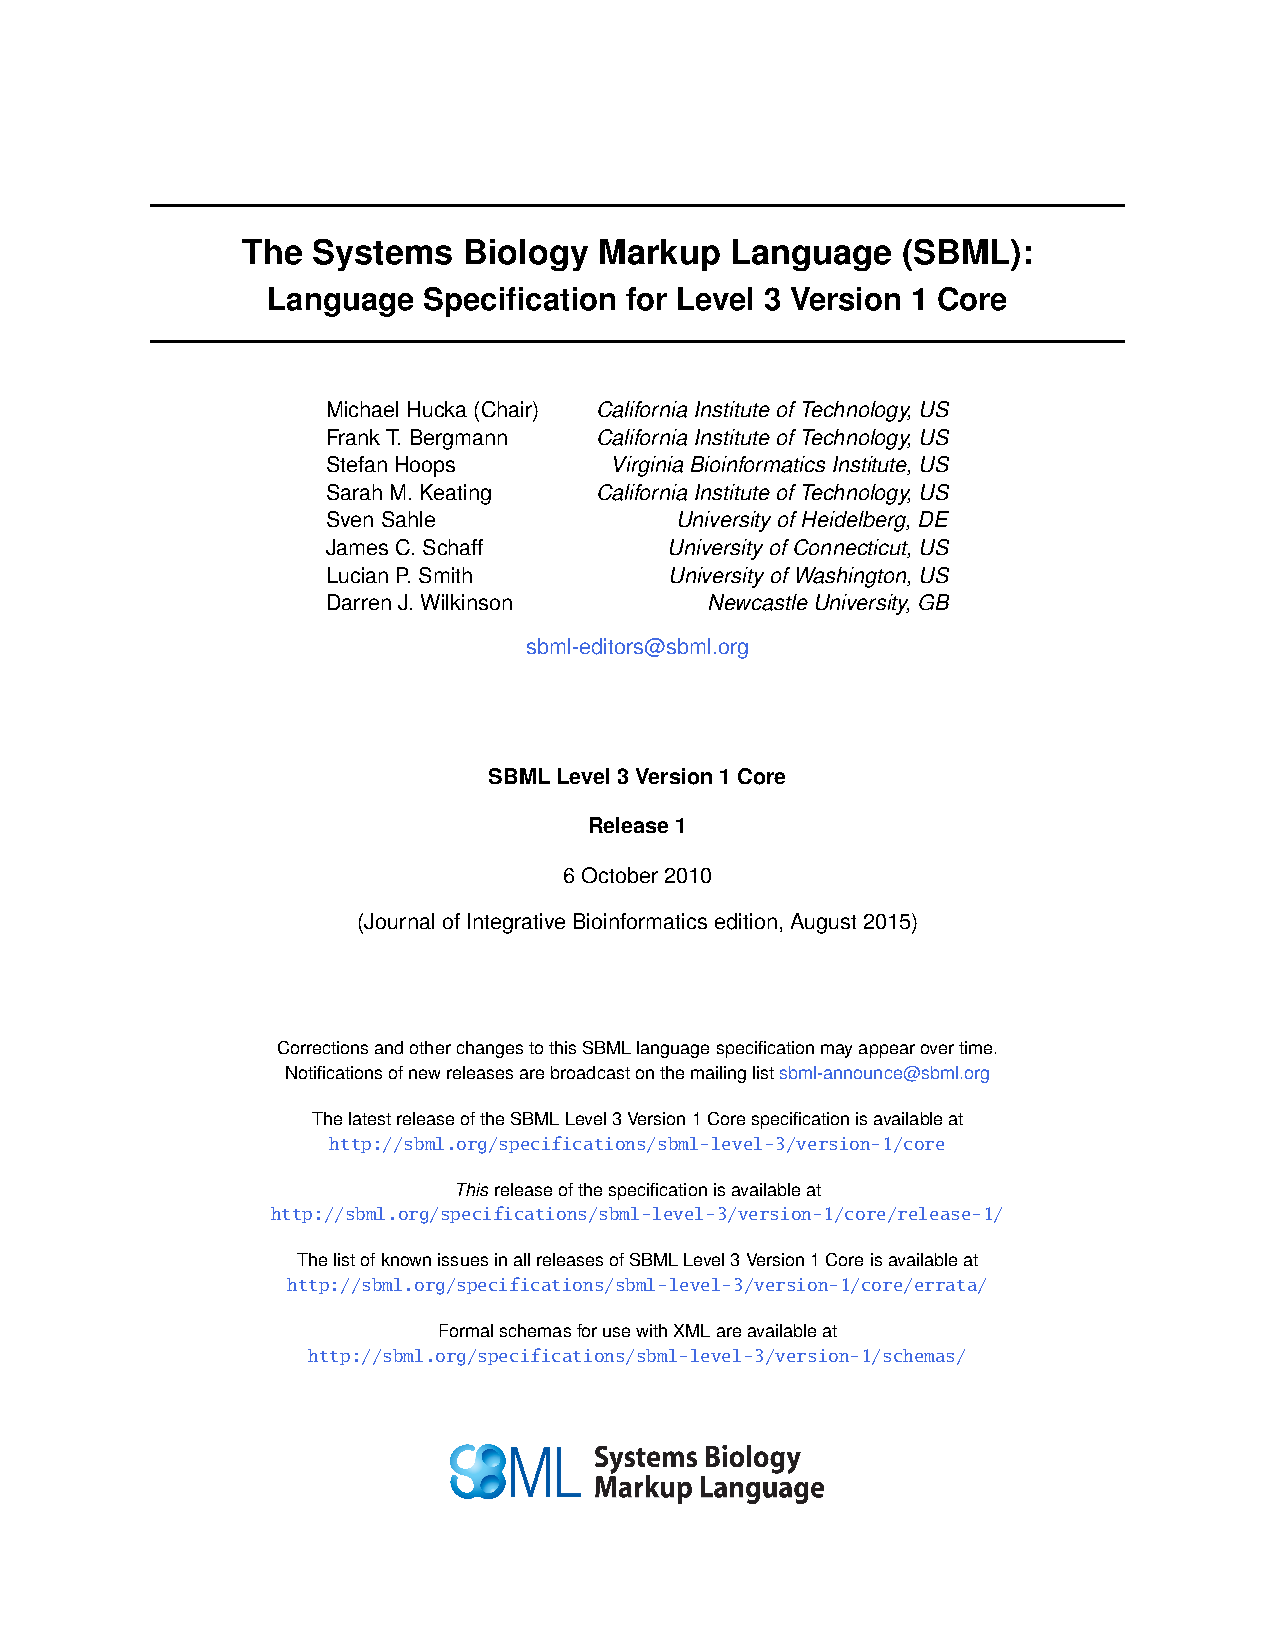
\includepdf[pages=-]{../spec/sbml-level-3-version-1-core.pdf}

\end{document}
